\documentclass[11pt,a4paper]{article}
\usepackage[margin=1in]{geometry}
\usepackage{amsmath,graphicx,float,booktabs,listings,fancyhdr}
\usepackage{xcolor}
\usepackage[hidelinks]{hyperref}
\newcommand{\remaining}[1]{\par\noindent\textcolor{red}{Still needed: #1}\par}
\setcounter{secnumdepth}{0}
\setcounter{tocdepth}{2}
\pagestyle{fancy}
\fancyhf{}
\fancyhead[L]{Signals \& Systems Lab 5}
\fancyfoot[C]{\thepage}
\setlength{\headheight}{14.5pt}
\lstset{language=Python,basicstyle=\ttfamily\footnotesize,
    breaklines=true,showstringspaces=false,keepspaces=true,
    columns=fullflexible,tabsize=4}
\graphicspath{{Lab_5/Python/}{Python/}{../Python/}}
\begin{document}

\begin{titlepage}
    \vspace*{2cm}
    \centering
    {\huge Signals and Systems Lab 5\par}
    \vspace{0.5cm}
    {\Large Communication Systems: Amplitude Modulation and Demodulation\par}
    \vspace{0.5cm}
    {\large Liam Donlan, Colden Briggs, Eben Radocchia\par}
    \vspace{0.3cm}
    {\large \today\par}
\end{titlepage}

\tableofcontents
\newpage

\section{Introduction}

This lab studied how modulation sends two audio messages over one channel and how demodulation, filtering, and carrier phase affect their recovery.

\section{Part 1: Multiplexing Two Messages}

\subsection{Task 1.1: Band-Limit the Two Clips}

\subsubsection{Code}
\begin{lstlisting}
import numpy as np
import matplotlib
matplotlib.use("Agg")
import matplotlib.pyplot as plt
from scipy.io import wavfile
from scipy.signal import fftconvolve

fs = 44100
W = 2000
f1 = 6000
f2 = 12000

def plot_spectrum(x, fs, fmax, title):
    N = len(x)
    X = np.abs(np.fft.rfft(x * np.hanning(N)))
    f = np.fft.rfftfreq(N, 1.0 / fs)
    X = X / np.max(X)
    keep = f <= fmax
    plt.figure(figsize=(7, 3))
    plt.plot(f[keep], X[keep], lw=0.8)
    plt.xlabel("frequency (Hz)")
    plt.ylabel("|X| (normalized)")
    plt.title(title)
    plt.tight_layout()
    plt.savefig(title.replace(" ", "_") + ".png")
    plt.close()

def ideal_lowpass(x, fs, cutoff):
    X = np.fft.rfft(x)
    f = np.fft.rfftfreq(len(x), 1.0 / fs)
    X[f > cutoff] = 0.0
    return np.fft.irfft(X, n=len(x))

def save_audio(filename, y):
    y = y / np.max(np.abs(y))
    y_i16 = np.int16(np.clip(y, -1, 1) * 32767)
    wavfile.write(filename, fs, y_i16)

sr1, m1raw = wavfile.read("clip1.wav")
sr2, m2raw = wavfile.read("clip2.wav")
assert sr1 == sr2 == fs
m1raw = m1raw.astype(float)
m2raw = m2raw.astype(float)
if m1raw.ndim > 1:
    m1raw = m1raw.mean(axis=1)
if m2raw.ndim > 1:
    m2raw = m2raw.mean(axis=1)
N = min(len(m1raw), len(m2raw))
m1raw, m2raw = m1raw[:N], m2raw[:N]
t = np.arange(N) / fs

plot_spectrum(m1raw, fs, 8000, "Clip 1 Raw Waveform")
plot_spectrum(m2raw, fs, 8000, "Clip 2 Raw Waveform")

m1 = ideal_lowpass(m1raw, fs, W)
m1 = m1 / np.max(np.abs(m1))
m2 = ideal_lowpass(m2raw, fs, W)
m2 = m2 / np.max(np.abs(m2))

plot_spectrum(m1, fs, 8000, "Clip 1 Band-Limited Waveform")
plot_spectrum(m2, fs, 8000, "Clip 2 Band-Limited Waveform")
save_audio("band-limited_clip1.wav", m1)
save_audio("band-limited_clip2.wav", m2)
\end{lstlisting}

\subsubsection{Raw Spectra and Frequency Ranges}

For both clips, appreciable energy lies approximately within 0--4000 Hz, strongest below 2000 Hz, with weak nonzero content continuing to 8000 Hz in the plotted range.
\begin{figure}[H]
    \centering
    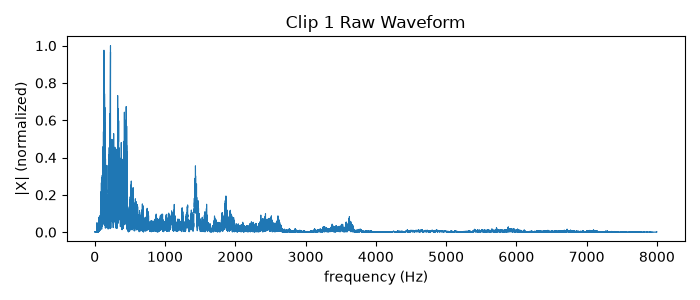
\includegraphics[width=0.9\linewidth]{Clip_1_Raw_Waveform.png}
    \caption{Magnitude spectrum of raw clip 1.}
\end{figure}
\begin{figure}[H]
    \centering
    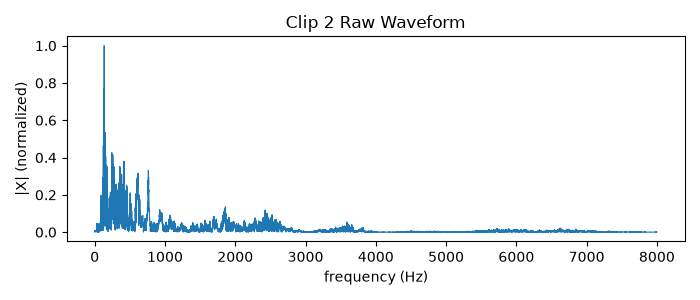
\includegraphics[width=0.9\linewidth]{Clip_2_Raw_Waveform.png}
    \caption{Magnitude spectrum of raw clip 2.}
\end{figure}

\subsubsection{Band-Limited Spectra and Confirmation of the 2000 Hz Cutoff}

Both filtered spectra show no visible energy above the 2000 Hz cutoff.
\begin{figure}[H]
    \centering
    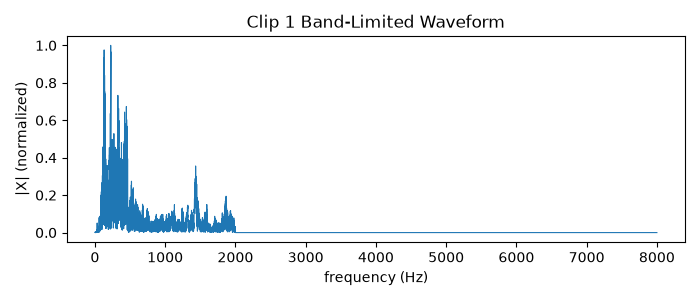
\includegraphics[width=0.9\linewidth]{Clip_1_Band-Limited_Waveform.png}
    \caption{Magnitude spectrum of clip 1 after ideal band-limiting.}
\end{figure}
\begin{figure}[H]
    \centering
    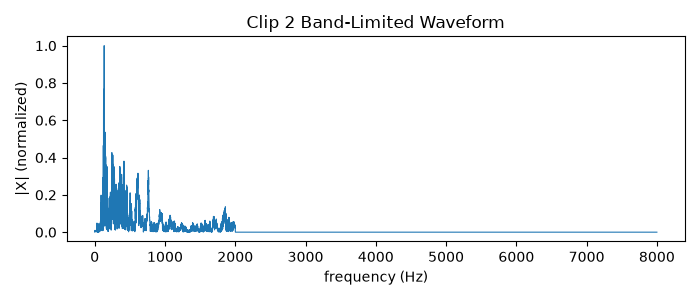
\includegraphics[width=0.9\linewidth]{Clip_2_Band-Limited_Waveform.png}
    \caption{Magnitude spectrum of clip 2 after ideal band-limiting.}
\end{figure}

\subsubsection{Listening Comparison}

\remaining{Listen to the raw and band-limited clips and add one sentence comparing their sound.}

\subsection{Task 1.2: Modulate}

\subsubsection{Derivation and Hand Sketch of \(X(j\omega)\)}

\remaining{Derive $X(j\omega)$ using the multiplication property and add the hand sketch of the shifted message spectra.}

\subsubsection{Frequency Band Edges}

\remaining{Give the lower and upper band edges in Hz for all four shifted spectral copies.}

\subsubsection{Carrier Spacing Condition and Verification}

\remaining{Derive the carrier-spacing condition and check it using the given bandwidth and carrier frequencies.}

\subsubsection{Code}
\begin{lstlisting}
c1 = np.cos(2 * np.pi * f1 * t)
c2 = np.cos(2 * np.pi * f2 * t)
x = m1 * c1 + m2 * c2
plot_spectrum(x, fs, 20000, "Transmitted Signal x(t) Waveform")
\end{lstlisting}

\subsubsection{Transmitted Spectrum and Comparison with Predicted Bands}

The numerical spectrum shows two separate bands centered on the assigned carriers, matching the expected band locations without visible overlap.
\begin{figure}[H]
    \centering
    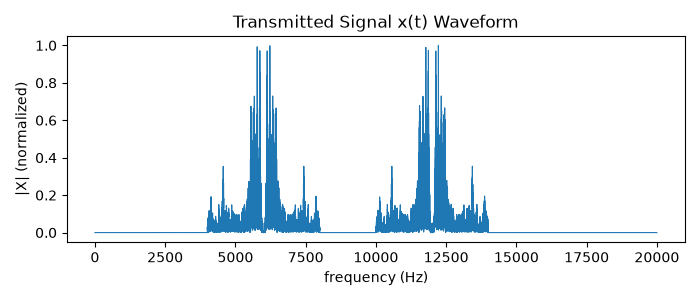
\includegraphics[width=0.9\linewidth]{Transmitted_Signal_x(t)_Waveform.png}
    \caption{Magnitude spectrum of the transmitted signal \(x(t)\).}
\end{figure}

\subsubsection{Why One Scalar Signal Carries Both Messages}

The messages occupy separate frequency bands, so they can be added into one signal and individually recovered by demodulation and filtering.

\newpage
\section{Part 2: Demodulation}

\subsection{Task 2.1: Demodulation}

\subsubsection{Four-Term Trigonometric Expansion}

\remaining{Substitute the transmitted signal into $r_1(t)$ and use trigonometric identities to obtain the four-term expansion.}

\subsubsection{Center Frequencies, Wanted and Unwanted Bands, and Lowest Unwanted Frequency}

The baseband band is wanted, and the three higher-frequency bands are unwanted.

\remaining{Give all four center frequencies in Hz and the lowest frequency among the unwanted bands.}

\subsubsection{Fourier Multiplication-Property Derivation and Hand Sketch}

\remaining{Derive and hand-sketch $R_1(j\omega)$ using the multiplication property and confirm its center frequencies match the trigonometric result.}

\subsubsection{Code}
\begin{lstlisting}
r1 = x * np.cos(2 * np.pi * f1 * t)
plot_spectrum(r1, fs, 20000, "Demodulated Channel 1 Spectrum")
\end{lstlisting}

\subsubsection{Demodulated Spectrum and Verification of the Four Bands}

The numerical spectrum shows one band at baseband and three at higher frequencies, consistent with the demodulation prediction.
\begin{figure}[H]
    \centering
    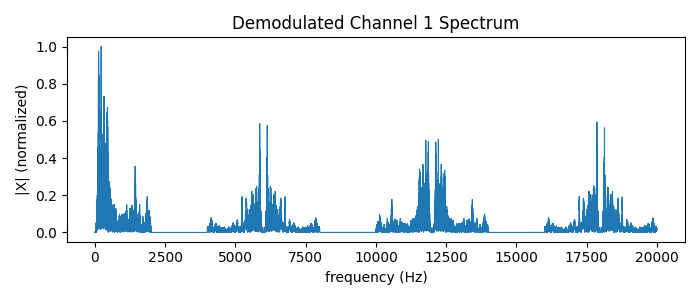
\includegraphics[width=0.9\linewidth]{Demodulated_Channel_1_Spectrum.png}
    \caption{Magnitude spectrum of \(r_1(t)=x(t)\cos(2\pi f_1t)\) before reconstruction.}
\end{figure}

\subsubsection{Why the Wanted Message Is at Baseband}

Mixing with the matching carrier shifts channel 1 to zero frequency, while channel 2 remains offset because its carrier frequency is different.

\newpage
\section{Part 3: Reconstruction with an Ideal Low-Pass Filter}

\subsection{Task 3.1: Recover Using a Low-Pass Filter}

\subsubsection{Hand Sketch of the Bands and Ideal Filter Response}

\remaining{Hand-sketch the four bands with labeled centers and widths, then overlay the ideal filter response with amplitude 2 and cutoff $W$.}

\subsubsection{Graphical Prediction of the Recovered Message}

\remaining{Use the convolution property to shade the surviving band and state the recovered message in terms of the original message.}

\subsubsection{Code for Recovering Both Channels}
\begin{lstlisting}
r2 = x * np.cos(2 * np.pi * f2 * t)
m1hat = 2 * ideal_lowpass(r1, fs, W)
m2hat = 2 * ideal_lowpass(r2, fs, W)
save_audio("reconstructed_clip1.wav", m1hat)
save_audio("reconstructed_clip2.wav", m2hat)

n = int(fs * 0.020)
plt.figure(figsize=(7, 3))
plt.plot(t[:n] * 1000, m1[:n], label="m1")
plt.plot(t[:n] * 1000, m1hat[:n], label="m1hat")
plt.xlabel("Time (ms)")
plt.ylabel("Amplitude")
plt.title("First 20 ms of m1 and m1hat")
plt.legend()
plt.tight_layout()
plt.savefig("m1_and_m1hat_Waveforms.png")
plt.close()
\end{lstlisting}

\subsubsection{20 ms Overlay of Original and Recovered Channel 1}
\begin{figure}[H]
    \centering
    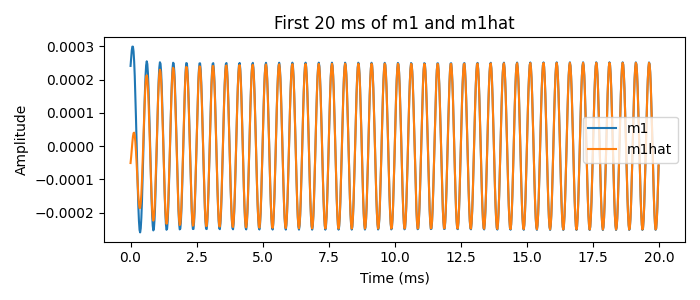
\includegraphics[width=0.9\linewidth]{m1_and_m1hat_Waveforms.png}
    \caption{The first 20 ms of band-limited \(m_1(t)\) and ideally reconstructed \(\hat m_1(t)\).}
\end{figure}

\subsubsection{Waveform and Listening Comparison}

The recovered and original waveforms nearly overlap, apart from a small mismatch near the start of the plotted segment.

\remaining{Play both ideally recovered channels and add a short sound comparison with the band-limited messages.}

\subsubsection{Explanation of Channel Separation}

The ideal filter keeps the baseband message and removes the channel-2 bands because they lie above its cutoff.

\subsection{Task 3.2: Phase Coherence}

\subsubsection{Derivation of the Recovered Baseband Term}

\remaining{Use the product-to-sum identity to derive the recovered baseband term for a phase-offset local carrier and show its phase dependence.}

\subsubsection{Code}
\begin{lstlisting}
rms_m1 = float(np.sqrt(np.mean(m1 ** 2)))
phase_rows = []
for phi in [0, 30, 60, 90]:
    phi_rad = np.deg2rad(phi)
    mixed = x * np.cos(2 * np.pi * f1 * t + phi_rad)
    y1hat = 2 * ideal_lowpass(mixed, fs, W)
    rms_y1 = float(np.sqrt(np.mean(y1hat ** 2)))
    predicted = rms_m1 * abs(np.cos(phi_rad))
    phase_rows.append((phi, np.cos(phi_rad), rms_y1, predicted))
    print(phi, rms_y1, predicted)
\end{lstlisting}

\subsubsection{RMS Table Compared with \(\cos\phi\)}
\begin{table}[H]
    \centering
    \begin{tabular}{rrrr}
        \toprule
        \(\phi\) (degrees) & \(\cos\phi\) & Measured RMS & \(\operatorname{RMS}(m_1)|\cos\phi|\) \\
        \midrule
        0  & 1.0000 & 0.117306 & 0.117306 \\
        30 & 0.8660 & 0.101590 & 0.101590 \\
        60 & 0.5000 & 0.058653 & 0.058653 \\
        90 & 0.0000 & \(2.19\times10^{-6}\) & 0 \\
        \bottomrule
    \end{tabular}
    \caption{RMS of the reconstructed signal after ideal low-pass filtering and multiplication by 2.}
\end{table}

\subsubsection{The \(90^\circ\) Result and Receiver Carrier Requirements}

At a $90^\circ$ phase offset, the desired baseband component cancels and the measured RMS is nearly zero, so the receiver needs a carrier matched in frequency and phase.

\newpage
\section{Part 4: Reconstruction with the Two-Stage RC Network}

\subsection{Task 4.1: The RC Network at Both Ends and Comparison}

\subsubsection{RC and Ideal Frequency Response Overlay}
\begin{figure}[H]
    \centering
    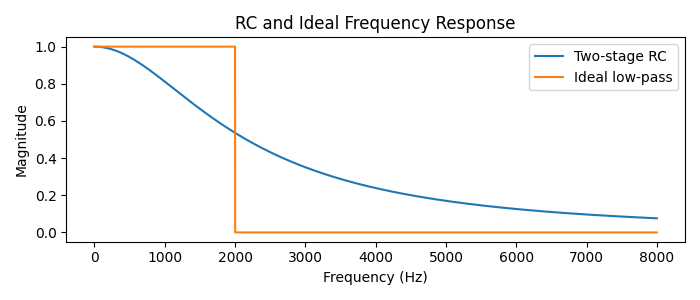
\includegraphics[width=0.9\linewidth]{RC_and_Ideal_Frequency_Response.png}
    \caption{Magnitude responses of the two-stage RC network and the ideal low-pass filter with a 2000 Hz cutoff.}
\end{figure}

\subsubsection{Explanation of Frequency Response Differences}

The ideal filter has a flat passband and an abrupt cutoff, while the RC response decreases gradually and attenuates some message frequencies.

\subsubsection{Hand Sketches of RC Modulation and Demodulation}

\remaining{Add hand sketches showing how RC filtering changes the modulation and demodulation spectra relative to the ideal chain, using the convolution and multiplication properties.}

\subsubsection{Transmit Band Overlap, Partial Receive Rejection, and Channel Leakage}

The RC transmit filter leaves high-frequency tails, so the modulated spectra overlap, and the receive filter only attenuates the unwanted bands, allowing channel 2 to leak into channel 1.

\subsubsection{Code for the RC Impulse Response and Both Transmit and Receive Filters}
\begin{lstlisting}
R1, C1 = 10e3, 10e-9
R2, C2 = 4.7e3, 10e-9
tau1 = R1 * C1
tau2 = R2 * C2
G = 1

f = np.linspace(0, 8000, 4001)
Hrc = G / ((1 + 1j * 2 * np.pi * f * tau1)
           * (1 + 1j * 2 * np.pi * f * tau2))
Hideal = (f <= W).astype(float)
plt.figure(figsize=(7, 3))
plt.plot(f, np.abs(Hrc), label="Two-stage RC")
plt.plot(f, Hideal, label="Ideal low-pass")
plt.xlabel("Frequency (Hz)")
plt.ylabel("Magnitude")
plt.title("RC and Ideal Frequency Response")
plt.legend()
plt.tight_layout()
plt.savefig("RC_and_Ideal_Frequency_Response.png")
plt.close()

def h(t):
    t = np.asarray(t, dtype=float)
    y = np.zeros_like(t)
    keep = t >= 0
    y[keep] = G / (tau1 - tau2) * (
        np.exp(-t[keep] / tau1) - np.exp(-t[keep] / tau2))
    return y

sr1, raw1 = wavfile.read("clip1.wav")
sr2, raw2 = wavfile.read("clip2.wav")
assert sr1 == sr2 == fs
raw1, raw2 = raw1.astype(float), raw2.astype(float)
if raw1.ndim > 1:
    raw1 = raw1.mean(axis=1)
if raw2.ndim > 1:
    raw2 = raw2.mean(axis=1)
N = min(len(raw1), len(raw2))
raw1, raw2 = raw1[:N], raw2[:N]
t = np.arange(N) / fs
kernel = h(t) / fs

m1RC = fftconvolve(raw1, kernel)[:N]
m2RC = fftconvolve(raw2, kernel)[:N]
m1RC = m1RC / np.max(np.abs(m1RC))
m2RC = m2RC / np.max(np.abs(m2RC))

xRC = (m1RC * np.cos(2 * np.pi * f1 * t)
       + m2RC * np.cos(2 * np.pi * f2 * t))
r1RC = xRC * np.cos(2 * np.pi * f1 * t)
r2RC = xRC * np.cos(2 * np.pi * f2 * t)
m1RChat = 2 * fftconvolve(r1RC, kernel)[:N]
m2RChat = 2 * fftconvolve(r2RC, kernel)[:N]

save_audio("RC_reconstructed_clip1.wav", m1RChat)
save_audio("RC_reconstructed_clip2.wav", m2RChat)

plot_spectrum(m1hat, fs, 8000, "Clip 1 Reconstructed Waveform")
plot_spectrum(m2hat, fs, 8000, "Clip 2 Reconstructed Waveform")
plot_spectrum(m1RChat, fs, 8000, "Clip 1 RC Reconstructed Waveform")
plot_spectrum(m2RChat, fs, 8000, "Clip 2 RC Reconstructed Waveform")
\end{lstlisting}

\subsubsection{Listening Comparison with Both Ideal Recoveries and Channel 1 Intelligibility}

\remaining{Listen to both RC recoveries, compare them with the ideal recoveries, and state whether the channel-1 message remains audible.}

\subsubsection{RC and Ideal Recovered Magnitude Spectra up to 8 kHz}
\begin{figure}[H]
    \centering
    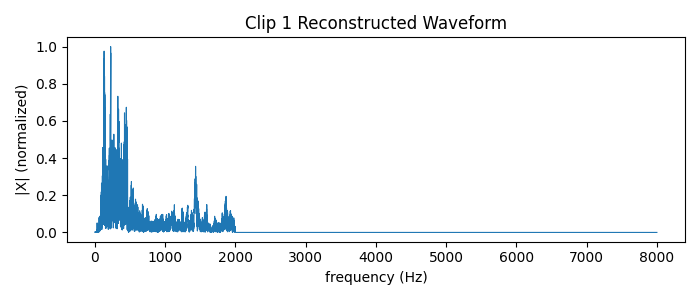
\includegraphics[width=0.9\linewidth]{Clip_1_Reconstructed_Waveform.png}
    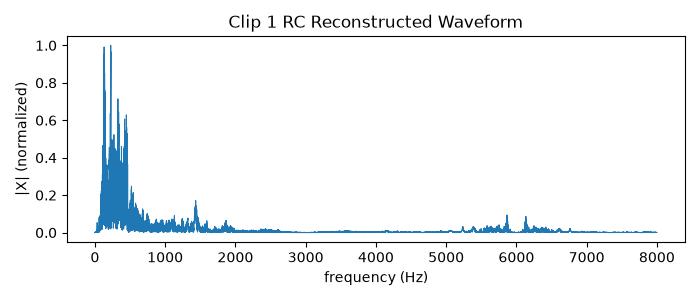
\includegraphics[width=0.9\linewidth]{Clip_1_RC_Reconstructed_Waveform.png}
    \caption{Channel 1 recovered magnitude spectra for the ideal chain (top) and RC chain (bottom). Each spectrum is normalized to its own peak.}
\end{figure}
\begin{figure}[H]
    \centering
    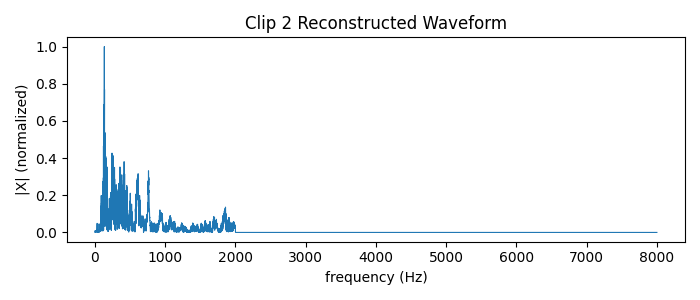
\includegraphics[width=0.9\linewidth]{Clip_2_Reconstructed_Waveform.png}
    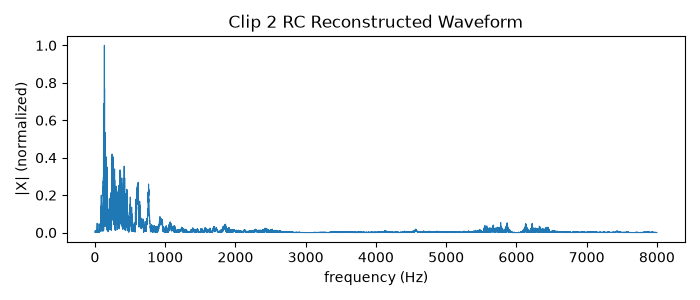
\includegraphics[width=0.9\linewidth]{Clip_2_RC_Reconstructed_Waveform.png}
    \caption{Channel 2 recovered magnitude spectra for the ideal chain (top) and RC chain (bottom). Each spectrum is normalized to its own peak.}
\end{figure}

\subsubsection{Explanation of Spectral Differences}

Compared with the ideal recoveries, the RC recoveries have weaker upper message frequencies relative to low frequencies and residual peaks above 2000 Hz because the RC filter rolls off gradually.

\subsubsection{Reducing Leakage by Changing Carrier Frequencies and RC Time Constants}

Increase the carrier spacing and use larger RC time constants for stronger rejection, while allowing enough bandwidth to retain the messages.

\newpage
\section{Conclusion}

Modulation placed two messages in separate frequency bands, and coherent demodulation with ideal filtering recovered them. Phase errors weakened recovery, while RC filtering attenuated higher message frequencies and allowed channel leakage.

\end{document}